\question 某机器字长为8位,采用原码表示法(其中一位为符号位),则机器数所能表示的范围是(
~)
\par\fourch{\textcolor{red}{-127~+127}}{-127~+128}{-128~+127}{-128~+128}
\begin{solution}假设机器数字长为n位,包含一位符号位,则原码、补码、反码的表示范围见下表。

~
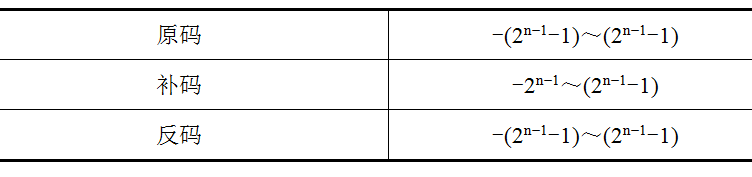
\includegraphics[width=3.33333in,height=0.81250in]{computerassets/F9B4A5C57401D2BDF1DB8B2987BCD52F.png}
\end{solution}
\question 下列数中最小的数为
\par\twoch{\textcolor{red}{BIN:10010101}}{OCT:227}{DEC:177}{HEX:96}
\begin{solution}``BIN''表示二进制,``OCT''表示八进制。``DEC''表示十进制,``HEX''表示十六进制。
A.BIN:10010101 转换为DEC:149 B.OCT:227 转换为DEC:151 C.DEC:152
转换为DEC:152 D.HEX:96 转换为DEC:150 所以本题的答案为A。
\end{solution}
\question 计算机中表示地址时,采用
\par\twoch{原码}{补码}{移码}{\textcolor{red}{无符号数}}
\begin{solution}D。由于地址都是正数,肯定不需要浪费1bit来表示符号位,故采取无符号数来表示内存的地址,故选D。
\end{solution}
\question 在整数定点机中,下列说法正确的是
\par\fourch{原码和反码不能表示-1,补码可以表示-1}{\textcolor{red}{3种机器数均可表示-1}}{原码和补码不能表示-1,反码可以表示-1}{都不能表示-1}
\begin{solution}B。
首先考生需要看清楚题目,不然会误选A;题目说的是在整数定点机,那肯定是原码、补码、反码都可以表示-1,故选B。如果此题说的是在小数定点机,则应该选A。
\end{solution}
\question 4位机器内的数值代码,它所能表示的十进制真值为
\par\twoch{\textcolor{red}{15}}{-1}{-16}{以上三者均可能}
\begin{solution}A。
题目的意思很清楚,4位均为数值位,说明不包含符号位,也就是说为无符号数,故可以排除负数的可能。4位机器内的数值代码表示范围为0~15。
\end{solution}
\question 十进制数-0.3125的8位移码编码为
\par\twoch{D8H}{\textcolor{red}{58H}}{A8H}{28H}
\begin{solution}B。 首先写出0.3125的二进制表示形式为1010
1000(首位为符号位,小数点隐藏在符号位之后),然后可以直接写出补码的表示形式为1101
1000,移码即为补码的符号位取反,即0101 1000,转换成十六进制数为58H。
\end{solution}
\question 设x为整数,{[}x{]}补=1,x1x2x3x4x5,若要x小于-16,x1~x5应满足的条件是
\par\twoch{x1~x5至少有一个为1}{x1必须为1,x2~x5至少有一个为1}{x1必须为0,x2~x5至少有一个为1}{\textcolor{red}{x1必须为0,x2~x5任意}}
\begin{solution}D。
首先-16的补码是1,10000(第一个1为符号位),再次引用该结论:当使用补码表示时,如果符号位相同,则数值位越大,码值越大。因此,要使得x小于-16,第一位必须为0,后面则可以任意,即1,0XXXX,故选D。
\end{solution}
\question 某机字长8位,含一位数符,采用原码表示,则定点小数所能表示的非零最小正数为
\par\fourch{}{}{\textcolor{red}{}}{}
\begin{solution}C。
求最小的非零正数,符号位为0,数值位取非0中原码最小值,该8位数据编码为0.0000001,表示的值是2\^{}-7,所以选C。
\end{solution}
\question 已知{[}X{]}补=0.111 1110,则{[}X{]}原等于
\par\twoch{0.000 0001}{0.000 0010}{\textcolor{red}{0.111 1110}}{1.111 1110}
\begin{solution}C。
若原码的真值大于等于0,其补码跟原码一样。(注意原码中0有两种表示,但补码只有一个。对于原码中的两种0,无论用两种转换规则的哪种,其补码刚好都是一样的)
补码0.111 1110,从符号位得出为正数,其补码跟原码一样,故选C。
若为负数,其原码为``符号位不变,数值位取反,末位加1''。
\end{solution}
\question 相同位数的补码、移码、反码中,能表示的整数最多的是
\par\twoch{补码}{移码}{反码}{\textcolor{red}{补码和移码}}
\begin{solution}D。
四种表示方式中,正负数都是可以一一对应的。表示个数的差别就在于0的表示。
原码:原码的0有两种表示,即符号位为0和1两种零。
反码:正数的反码与其原码相同;负数的反码是对其原码逐位取反,但符号位除外。故反码的0也有两种表示。
补码:补码的0只有一种表示,形如0 0\ldots{}0,注意1
0\ldots{}0表示的不是负零,而是最大负数。
移码:移码是符号位取反的补码,故0也是只有一种表示。
通过对定义,理解四种表示方式之间的联系,万变不离其宗,很多时候就可以减少记忆错误的失分。
综上所述,补码和移码的表示整数个数都比原码和反码多1,故选D。
\end{solution}
\question 下列关于原码、补码、反码和移码的叙述中,不正确的是
\par\fourch{相同位数的补码和移码具有相同的数值范围}{零的补码和移码表示不同}{\textcolor{red}{一般反码用于表示浮点数的阶码}}{在实际计算机中,很少存储原码和反码}
\begin{solution}C。
同一真值的补码和移码只有一个符号位是不同的,且唐朔飞教材中有个真值、补码、移码的对照表。二者表示的范围是一样的。故A正确。
若机器字长k位,则{[}0{]}补=0 0\ldots{}0,{[}0{]}移=2\^{}k+0=1
0\ldots{}0,{[}0{]}补≠{[}0{]}移,故B正确。
一般移码用于表示浮点数的阶码,故C错误。 计算机一般存储的是补码和移码。
原码是有符号数的最简单的编码方式,便于输入输出,但很少用于存储。
反码一般是计算过程中的中间过程。 所以D的叙述也是正确的。
\end{solution}
\question n位补码可表示负数个数为
\par\fourch{}{}{}{\textcolor{red}{}}
\begin{solution}D。 n位补码表示整数的范围为{[}-2\^{}(n-1),
2\^{}(n-1)-1{]},其中负数为2\^{}(n-1)个。故选D。
\end{solution}
\question 计算机运算溢出检测机制,采用双符号位,下列关于双符号位的说法中正确的有(
) I. 00表示正号,11表示负号
II.结果的符号位为01时,称为上溢;为10时,称为下溢
III.符号位都为00的两个数相加,运算结果有可能产生溢出
IV.符号位都为11的两个数相加,运算结果不会产生溢出
\par\twoch{I}{I、II和IV}{I和IV}{\textcolor{red}{I、II和III}}
\begin{solution}I明显正确,这是规定。
II这个我们可以举例进行检验,比如举个上溢的例子,两个比较大的正整数相加,如00
1100 + 00 1100 = 01 1000。还可以举个下溢的例子,故II正确。
III正确,当两个同符号的数相加(或者是相异符号数相减)时,运算结果有可能产生溢出。
IV错误,解释如上。 故本题选D。
\end{solution}
\question 假定某数x=-0100 1010B,在计算机内部的表示为0011
0110B,则该数所用的编码方法是
\par\twoch{原码}{反码}{补码}{\textcolor{red}{移码}}
\begin{solution}D。 x=-0100 1010B,则x的原码为1100 1010,反码为1011 0101,补码为1011
0110,移码为0011 0110。原码、反码、补码和移码的转换总结见下图:
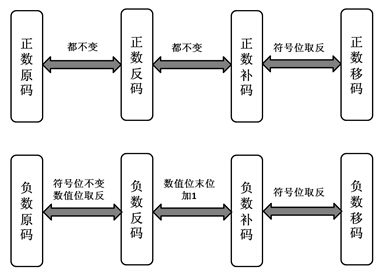
\includegraphics[width=4.00000in,height=2.88542in]{computerassets/ff87fd74ad5ca4f839ef07dc5dff3a95.jpeg}
\end{solution}
\question 用补码双符号位表示的定点小数,下述哪种情况属负溢出
\par\twoch{11 1111100}{01 0000100}{\textcolor{red}{10 0011000}}{00 1000000}
\begin{solution}C。 记住下面两句话即可。
①无论溢出与否,第一符号位始终表示的是结果的正确符号。
②若进位将会导致符号位不一致,就是表示溢出,反之就是没有溢出。
从这两句话,我们就可以判断出: 11符号表示------无溢出且符号为负。
01符号表示------正溢出。 10符号表示------负溢出。
00符号表示------无溢出且符号为正。 因此,易得C为负溢出的情况。
\end{solution}
\question 设寄存器位数为8位,机器数采用补码形式(含1位符号位)。对应于十进制数-27,寄存器内容为
\par\twoch{27H}{9BH}{\textcolor{red}{E5H}}{5AH}
\begin{solution}C。 x=-27=10011011,{[}x{]}补=11100101=E5H。
\end{solution}
\question 下列关于机器零的说法,正确的是
\par\fourch{发生“下溢”时,浮点数被当作机器零,机器将暂停运行,转去处理“下溢”}{\textcolor{red}{只有以移码表示的阶码时,才能用全0表示机器零的阶码}}{机器零属于规格化的浮点数}{定点数中的零也是机器零}
\begin{solution}B。
当浮点运算结果在0到最小正数之间(正下溢)或最大负数到0之间(负下溢)时,浮点数值趋于0,计算机仅将其当作机器零处理。
只有当数据发生``上溢''时,才会终止运算操作,转去进行溢出处理,A错误;规格化后可以判断运算结果是否上溢出(超过表示范围),但和机器零没有关联,C错误;定点数中所表示的0,是实实在在的0(坐标轴上的),而不是趋近0的机器零,D错误;在各种数码的表示法中,移码相当于真值在坐标轴上整体右移至正区间内,当移码表示的阶码全0时,为阶码表示的最小负数,此时直接认为浮点数是机器零,B正确。
\end{solution}
\question 将一个十进制数-8196表示成补码时,至少需采用( )位二进制代码表示
\par\twoch{12}{13}{14}{\textcolor{red}{15}}
\begin{solution}D。
n位补码(包括1位符号位)的表示范围是-2\^{}(n-1)~(2\^{}(n-1)-1),-2\^{}14(-16384)小于-8196小于-2\^{}13(-8192)。
故至少需要15位二进制代码表示。
\end{solution}
\question 下面的代码是一个C语言函数,用来计算两个长为len(len小于1000)的数组a和数组b对应元素的和,结果保存在数组c中,其中c{[}i{]}=a{[}i{]}+b{[}i{]}。当len为0时,返回值应该是空数组,但在执行时,却提示``Runtime
Error:Segmentation
fault''。后经检查是一个语句有误,改后就正常执行了。这个语句可能是 double
*sum\_array(double A{[}{]},double B{[}{]},unsigned int len) //① \{ int
i; //② double C{[}1000{]}; //③ for(i=0;i小于等于len-1;i++) //④ C{[}i{]}
= A{[}i{]}+B{[}i{]}; //⑤ return C; //⑥ \}
\par\twoch{①}{③}{④}{\textcolor{red}{①或④}}
\begin{solution}D。 Segmentation
fault,段错误就是访问了错误的内存段,一般是你没有权限,或者根本就不存在对应的物理内存。内存访问异常是由于对数组A,B访问时产生了越界错误而造成的。循环变量是int型的,而len是unsigned
int型,当len为0时,执行len-1的结果为FFFF
FFFF,是最大的可表示的32位无符号数,任何无符号数都比它小,使得数组越界访问,因而发生Segmentation
fault。 可以通过修改参数len的声明为int型,就能避免这一错误。
也可以将for(i=0;i小于等于len-1;i++)中的i小于等于len-1改为i
\end{solution}
\question 早期的计算机只有定点数表示,相比浮点数表示,定点数的缺点有
I.硬件结构复杂 II.运算编程困难 III.表示数的范围小
IV.数据存储单元的利用率很低
\par\twoch{I和II}{II和III}{III和IV}{\textcolor{red}{II、III和IV}}
\begin{solution}D。 浮点数的硬件结构比定点数复杂,故I不是定点数的缺点。
定点数进行运算时,程序程序设计人员必须首先确定机器小数点的位置,并把所有参与运算的数据的小数点都对齐到这个位置上,然后机器才能正确进行运算。故II属于定点数的缺点。
定点数的表示数范围小,16位字长的计算机所能表示的整数的范围只有-32768到32767。为了表示两个大小相差很大的数据,需要有很长的字长。故III属于定点数的缺点。
为了把小数点的位置定在数据最高位前面,必须把所有参与运算的数据至少都除以这些数据中的最大数,只有这样才能把所有数据都化成纯小数,因而会造成很多数据有大量的前置零,从而浪费了很多数据存储单元,导致数据存储单元的利用率很低。故IV属于定点数的缺点。
综上,本题选D。
\end{solution}
\question 在IEEE 754标准中,若存储阶码的寄存器中内容为3DH,则阶码对应的十进制数为
\par\twoch{61}{\textcolor{red}{-67}}{-61}{-66}
\begin{solution}B。 在IEEE754标准中,尾数采用原码表示,阶码部分采用移码表示。
故移码3DH,对应二进制为0011 1101,转换为补码为1011
1101,转换为原码为1100 0011,对应十进制为-67。选B。
\end{solution}
\question 一个C语言程序在一台32位机器上运行。程序中定义了三个变量x、y和z,其中x和z是int型,y为short型。当x=127,y=-9时,执行赋值语句z=x+y后,x、y和z的值分别是(
~)
\par\fourch{x=0000007FH,y=FFF9H,z=00000076H}{x=0000007FH,y=FFF9H,z=FFFF0076H}{x=0000007FH,y=FFF7H,z=FFFF0076H}{\textcolor{red}{x=0000007FH,y=FFF7H,z=00000076H}}
\begin{solution}此题考查如下知识点: (1)在计算机中,机器数默认使用补码表示。
(2)符号位扩展问题。所有扩展位使用符号位填充,即正数用0填充,负数用1填充。例如,1001扩充成8位,可以写成11111001;0111扩充成8位,可以写成00000111。
(3)强制类型转换。如果一个运算符两边的运算数类型不同,先要将其转换为相同的类型,即较低类型转换为较高类型,然后再参加运算。
1)对于x。x为int型,说明x占32位的存储空间。127转换成二进制为0000 0000
0000 0000 0000 0000 0111
1111,对应的十六进制为0000007FH,故x的值为0000007FH。
2)对于y。y为short型,说明y占16位的存储空间。-9的二进制表示为1000 0000
0000 1001,因此-9的补码表示为1111 1111 1111
0111(符号位不变,其余位取反加1),对应的十六进制为FFF7H。
3)对于z。z=x+y,由于y为short型,而x为int型,所以需要将y强制类型转换为int,那么就需要对y进行符号位扩展,将其从16位扩展到32位。因为y为负数,所以符号位为1,故需要在y的前面添加16个1,就可以实现将y强制转换为int型,强制转换后y的十六进制表示为FFFFFFF7H。故z=x+y=0000007FH+FFFFFFF7H=00000076H(可转成二进制进行计算),最高位的进1舍去。
\end{solution}
\question 假定有4个整数用8位补码分别表示为r1=FEH,r2=F2H,r3=90H,r4=F8H。若将运算结果存放在一个8位寄存器中,则下列运算中会发生溢出的是(
)
\par\twoch{r1×r2}{\textcolor{red}{r2×r3}}{r1×r4}{r2×r4}
\begin{solution}本题看上去较为复杂,因为牵涉到乘法运算。但本题的考查目的在于对补码的范围和溢出的理解。补码的最高位是符号位,相乘中只参与正负运算;溢出就是无法表示得到的结果。因此,如果按照书本上的方式来算出每个结果再判定,肯定会浪费时间。快速的解题方法如下:
8位补码所表示的十进制范围为-128~+127,可把4个十六进制数全部转换为十进制,进行口算相乘(适合数字很小的运算),得出的结果中,最大的就是会溢出的。
r1=FEH=1111 1110,符号位为1,说明为负数。除符号位取反加1,即1000
00010,故r1=--2。同理可得,r2=-14,r3=-112,r4=-8,故: r1×r2=28
r2×r3=1568 r1×r4=16 r2×r4=112 因此,只有r2×r3超出了范围-128~+127。
提醒:对于此种类型的题目,最重要的还是对于基础的掌握,对各种进制的转换要熟悉,并且对各种码制所能表达的范围要理解透彻。
【总结】
原码、补码、反码、移码的表示范围见下表。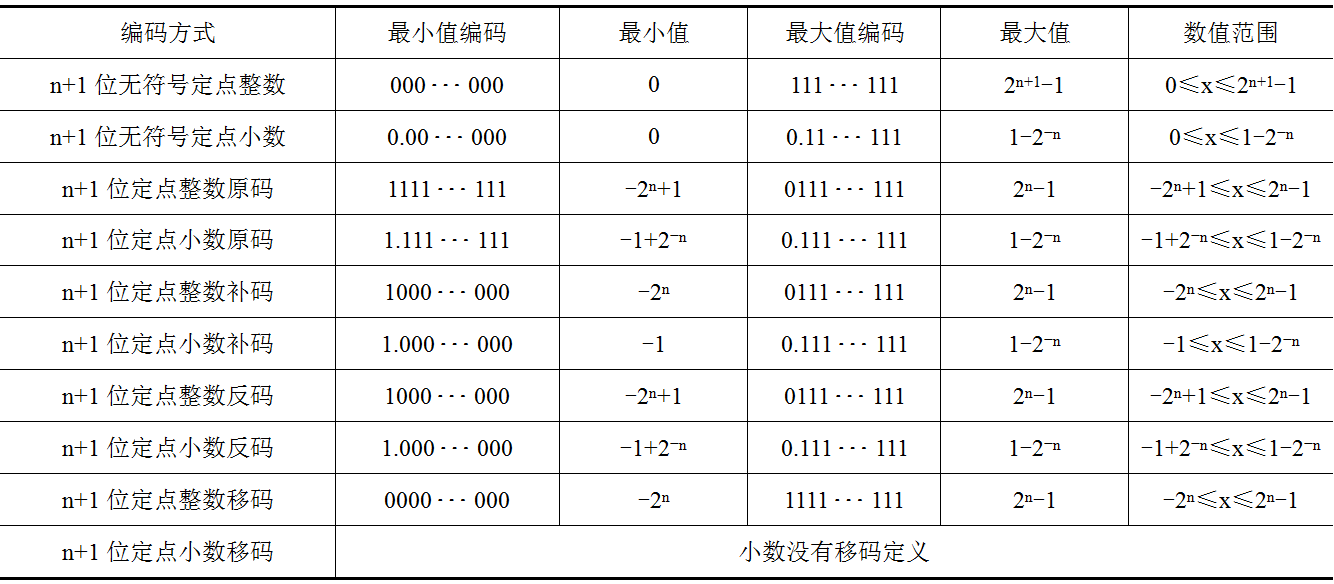
\includegraphics[width=3.46875in,height=1.52083in]{computerassets/0DC0AD3753DD835E184D090930E7A18E.png}
\end{solution}
\question 假设编译器规定int和short类型长度分别为32位和16位,若有下列C语言语句:
unsigned short x=65530; unsigned int y=x; 得到y的机器数为( )
\par\twoch{0000 7FFAH}{\textcolor{red}{0000 FFFAH}}{FFFF 7FFAH}{FFFF FFFAH}
\begin{solution}此题考查如下两个知识点:
(1)如何快速地将65530转换成十六进制?这里主要考查考生的一个逆向思维过程。考生应该记住对于16位无符号整数的最大值为65535(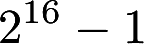
\includegraphics[width=0.52083in,height=0.16667in]{texmath/6c24d85Cdpi7B3507D25E7B167D-1}),其十六进制为FFFFH,那么就可以很轻松地得到65530的十六进制为FFFAH(F-5=A)。
(2)无符号短整型转换成无符号整型只需在高位补0即可。所以,最终得到y的机器数为y=0000
FFFAH。
\end{solution}
\question 某计算机有16个通用寄存器,采用32位定长指令字,操作码字段(含寻址方式位)为8位,Store指令的源操作数和目的操作数分别采用寄存器直接寻址和基址寻址方式。若基址寄存器可使用任一通用寄存器,且偏移量用补码表示,则Store指令中偏移量的取值范围是(
)
\par\twoch{\textcolor{red}{-32768~+32767}}{-32767~+32768}{-65536~+65535}{-65535~+65536}
\begin{solution}本题考察的是指令的寻址方式,这题可以采用排除法直接排出B、D选项,因为无论偏移量占多少位,由于偏移量是用补码表示的,它比原码表示的数要多出一个,而且多出的这一个正是补码表示的最小值,所以要么是-32768,要么是-65536。题目中是32位指令,操作码8位(已经包含了寻址方式)源操作数采用寄存器直接寻址,故可以采用4位来标记使用哪个寄存器,目的操作数采用基址寻址,由于题目告诉可以使用任一通用寄存器,故需要采用4位来标记,所以偏移量所占位数=32-8-4-4=16位,故偏移量的取值范围是-32768\textasciitilde{}+32768(含1位符号位)。
【总结】在考场上有时候即使我们不能一步就算出结果,或者题目复杂的时候,可以抓住问题的一些细节来排出某些选项,这对我们分析余下的选项也是很有帮助的,另外指令的各种寻址方式也一定要掌握,这里的偏移量是对形式地址的另外一种表示。
\end{solution}
\question 某字长为8位的计算机中,已知整型变量x、y的机器数分别为{[}x{]}补=1
1110100,{[}y{]}补=1 0110000。若整型变量z=2*x+y/2,则z的机器数为( )
\par\twoch{\textcolor{red}{1 1000000}}{0 0100100}{1 0101010}{溢出}
\begin{solution}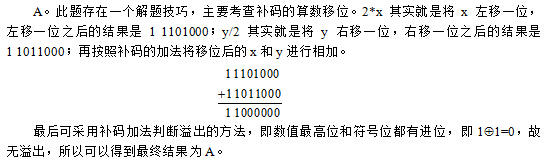
\includegraphics[width=5.73958in,height=1.75000in]{computerassets/f7aa3d33b4082cc7a9bf16eae72bd2a3.jpeg}
\end{solution}
